\chapter{Métodos Experimentales \label{cap:exp}}

En este capítulo se detallan los procedimientos experimentales desarrollados para la fabricación y caracterización de redes fotónicas basadas en guías de onda. La metodología comprende tres aspectos fundamentales: (1) escritura directa de guías mediante láser femtosegundo, (2) sistemas de excitación óptica con láser supercontinuo, y (3) técnicas avanzadas de modulación espacial de luz para el control de condiciones iniciales.


\section{Escritura directa de guías de onda \label{cap:fs}}

La fabricación de guías de onda se realizó mediante la técnica de escritura directa con láser femtosegundo: Pulsos ultracortos emitidos desde un láser de fibra Yb-dopado ATSEVA ANTAUS de 1030 nm, a una tasa de repetición de 500 kHz, son fuertemente enfocados en una muestra de borosilicato, produciendo cambios leves y permanentes en el índice de refracción local $\Delta n \sim 10^{-4}-10^{-3}$. Este método permite crear estructuras tridimensionales mediante movimientos controlados por computador de la plataforma XYZ Aerotech Nanopositioner \citep{femto_writing}.

\begin{figure}[H]
    \centering
    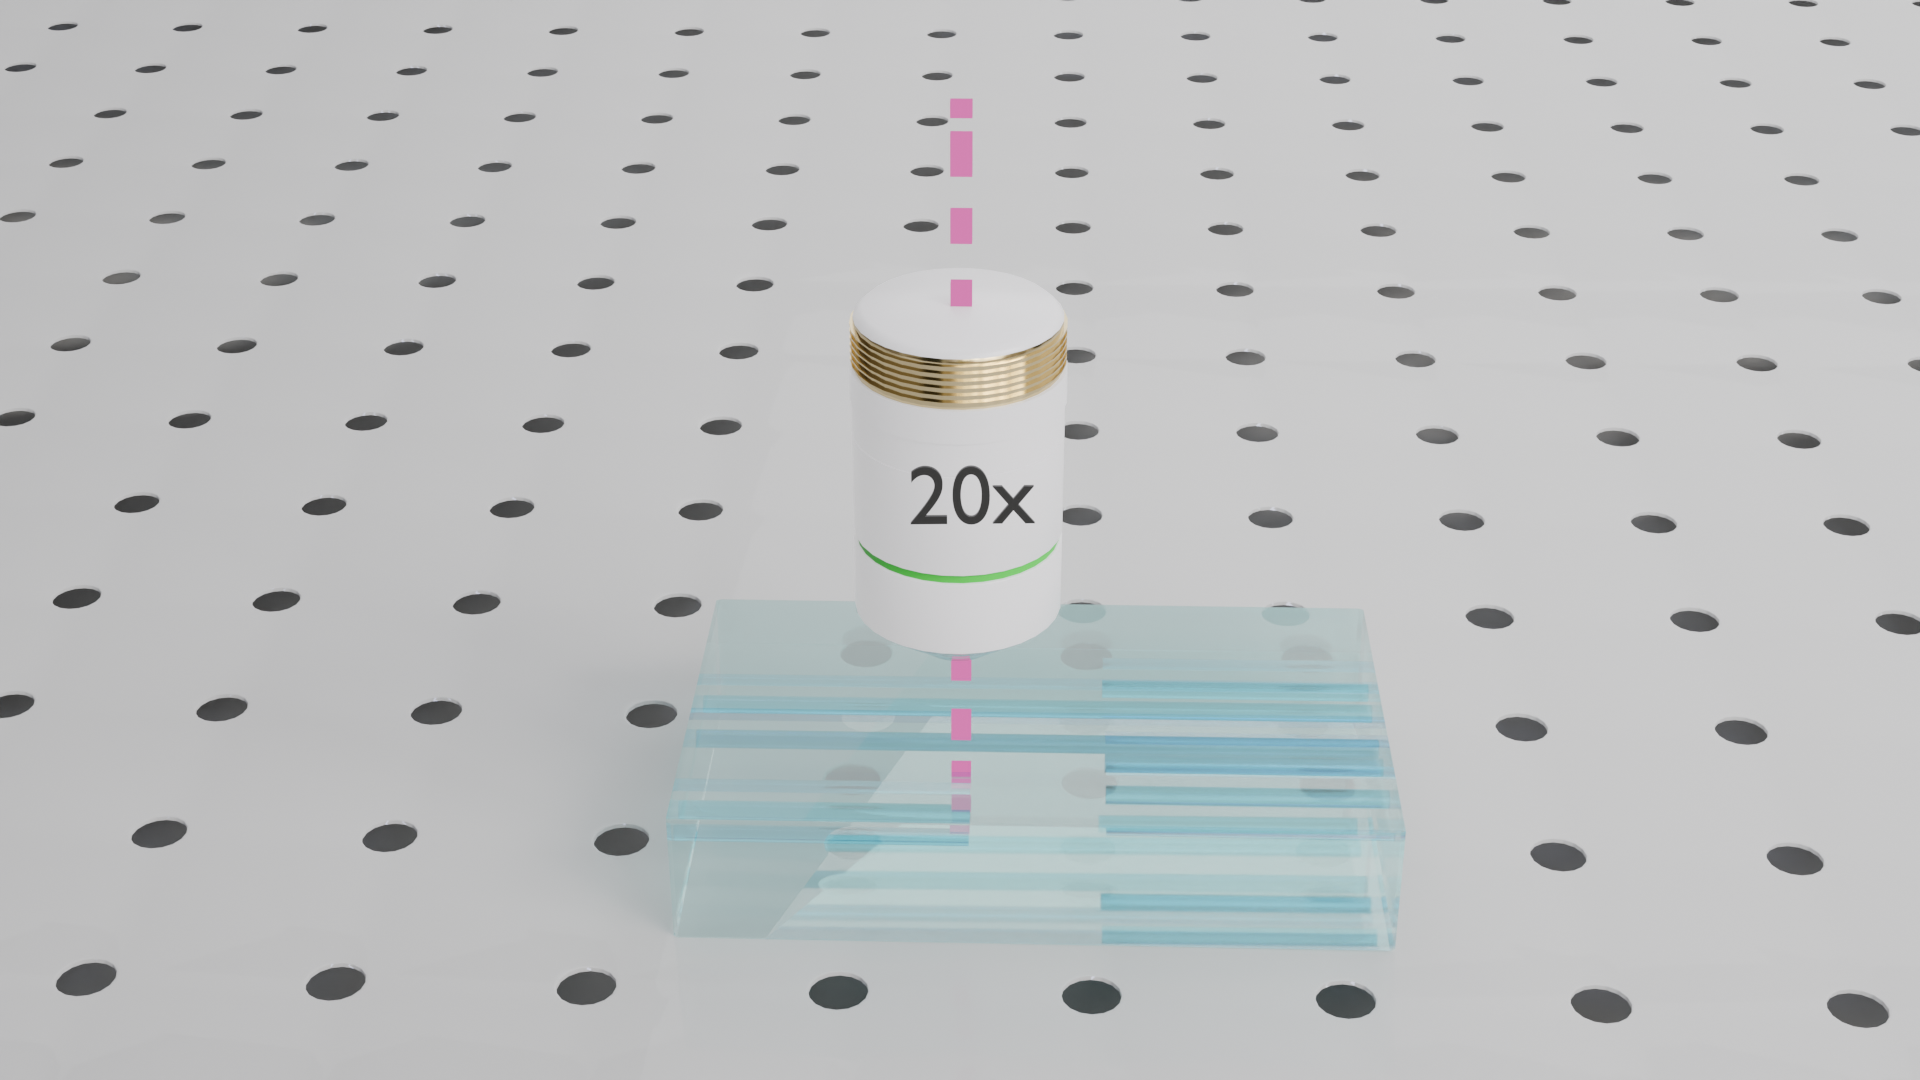
\includegraphics[width=0.6\linewidth, trim={18cm 4cm 15cm 6cm},clip]{media/fabrication1}
    \caption[Esquema de la técnica de escritura de guías de onda.]{Esquema de la técnica de escritura de guías de onda. El haz láser es focalizado mediante objetivo microscópico (20x) mientras la muestra se desplaza en tres ejes mediante una plataforma controlada por computadora.}
\end{figure}

Los parámetros de escritura que funcionan para excitar modos en el espectro visible son:
\begin{itemize}
	\item Ancho del pulso: 215 fs.
    \item Tasa de repetición: 500 kHz.
    \item Velocidad de escritura: 0.1 - 10.0 mm/s.
    \item Potencia de llegada medida: 90.0 - 144.0 mW.
\end{itemize}

\section{Montaje de excitación láser supercontinuo \label{cap:wavelength}}

Para la caracterización óptica se implementó un sistema de excitación basado en un láser supercontinuo (SC) de banda ancha (470nm to 2200nm). Específicamente, el modelo es un YSL SC-5. La configuración permite seleccionar longitudes de onda específicas mediante un modulador acústico AOTF-PRO (430 nm-1450 nm), con una resolución espectral de $\pm$5 nm y una potencia de salida de 1 mW por longitud de onda.

\begin{figure}[H]
    \centering
    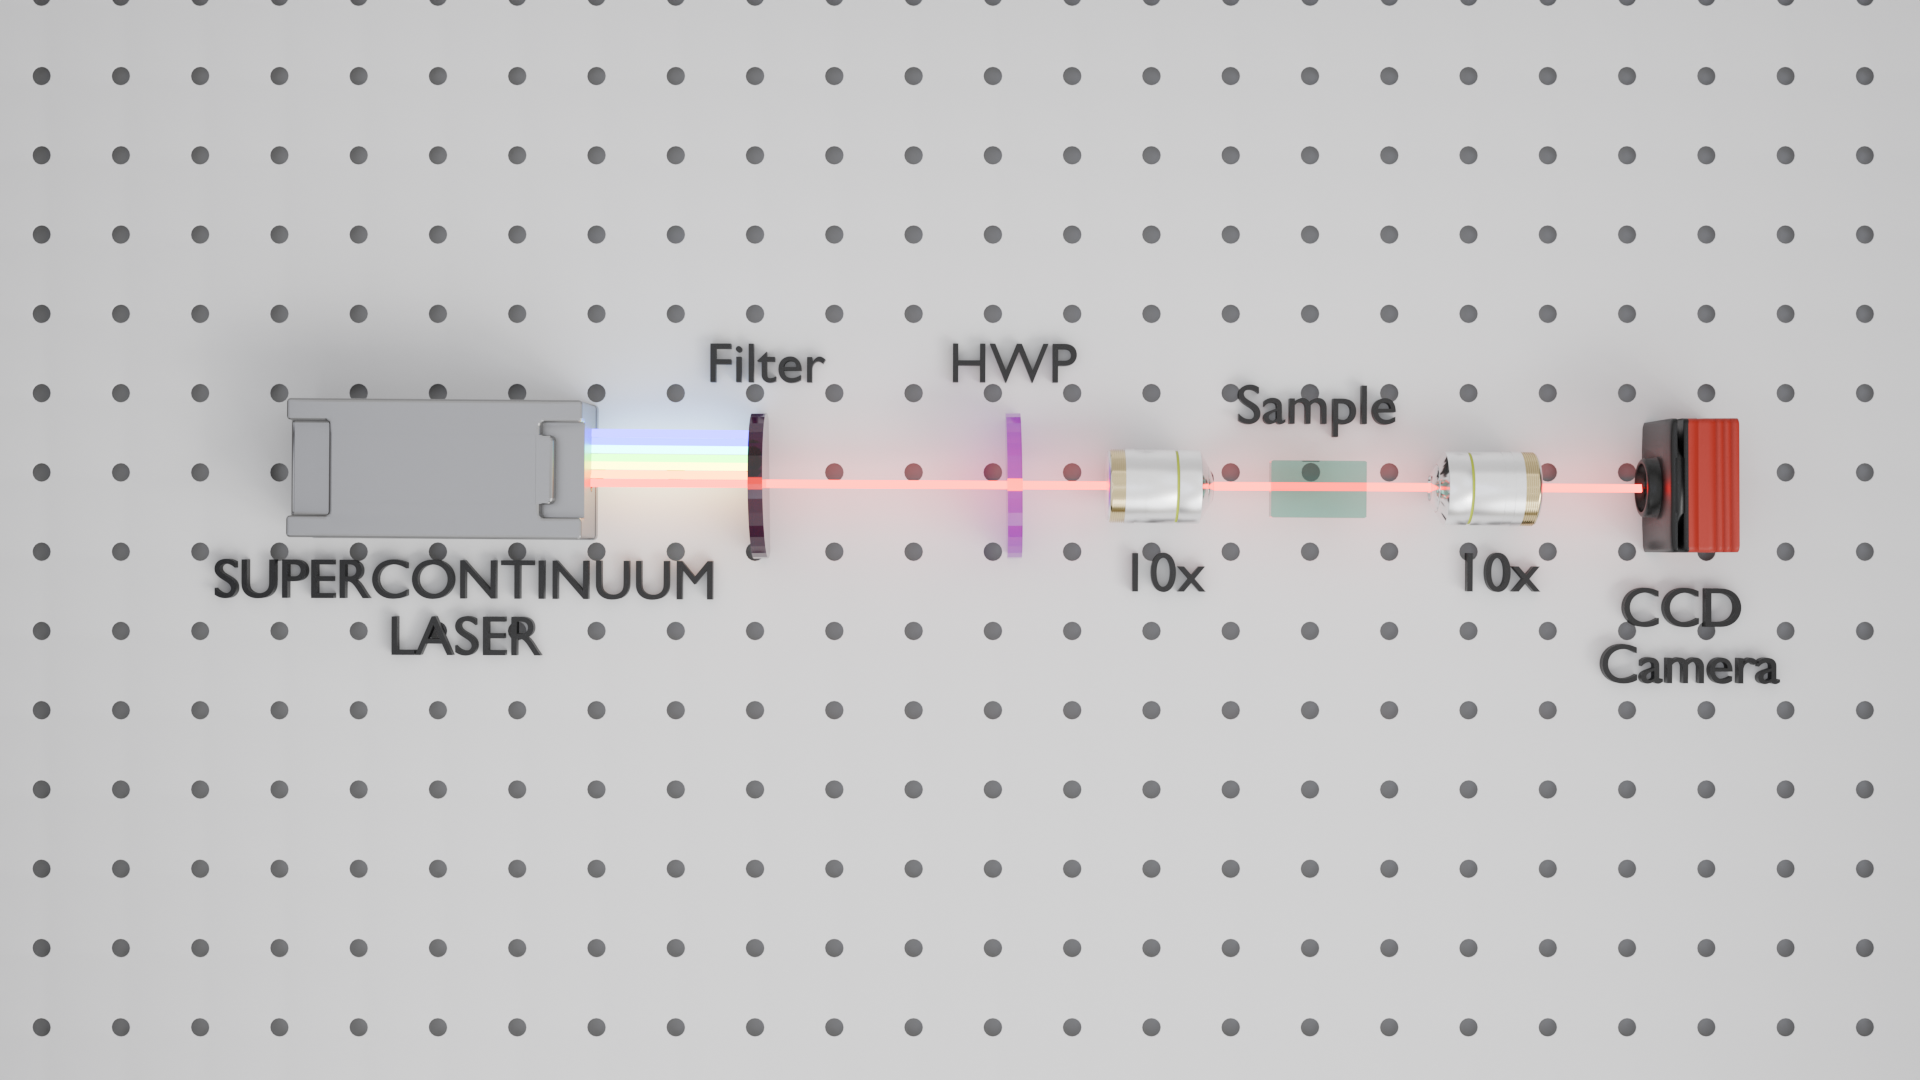
\includegraphics[width=\linewidth, trim={5cm 9cm 3cm 7cm},clip]{media/SC_setup}
    \caption[Montaje de excitación por láser supercontinuo.]{Montaje de excitación por láser supercontinuo. Filtro: Modulador acústico e iris. HWP: Retardador de media onda.}
\end{figure}

\section{Montaje de modulación espacial de luz}

Para usar condiciones iniciales distintas a una gaussiana se hace necesario incorporar métodos de modulación espacial de luz. En esta tesis se utilizó una técnica conocida como grabado de fase mediante holograma \citep{terhalle}.

\subsection{Etapa premodulación}
El modulador espacial de luz utilizado es un HOLOEYE PLUTO-NIR SLM - Reflective LCOS (resolución 1920$\times$1080 px, tamaño de píxel 8 $\mu$m), cuya respuesta óptica ocurre con polarización paralela al plano de la mesa óptica. Se utiliza un retardador de media onda ($\lambda/2$) seguido de un polarizador Glan-Thompson 100.000:1 con el objetivo de que la polarización de la luz láser coincida con la de la respuesta del SLM. Posteriormente se magnifica y se colima el haz para que abarque todo el área de pixeles disponible con un par de lentes 20x y $L_1$ de foco 100mm (telescopio). En la sección \ref{cap:oam} se muestra una aplicación del interferómetro.

\subsection{Etapa de modulación}
Una rejilla de difracción que maximiza la potencia del primer orden de difracción es utilizada. Para modular en amplitud se debe multiplicar la rejilla por la máscara de amplitud deseada, mientras que para modular en fase basta con sumar el nivel de gris correspondiente a la fase deseada. En la Figura \ref{fig:SLMblaze} se bosqueja el algoritmo implementado en Python en el anexo \ref{sec:codigoSLM}.

{
\sidecaptionvpos{figure}{c}
\begin{SCfigure}[]
    \centering
    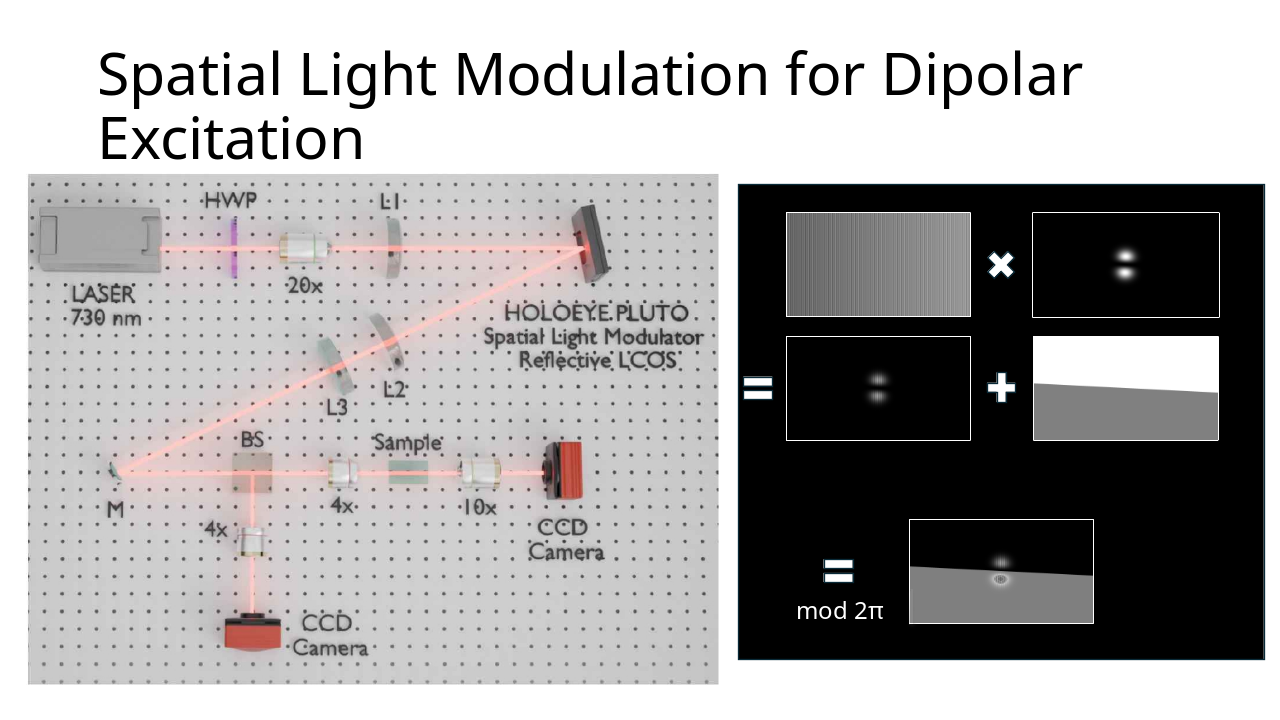
\includegraphics[width=0.35\linewidth, trim={19.5cm 0 0 5cm}, clip]{media/SLMblaze4.png}
    \caption[Modulación espacial de luz para máscaras de amplitud y fase arbitrarias.]{Algoritmo de modulación espacial de luz para máscaras de amplitud y fase arbitrarias. Los parámetros de la rejilla de difracción están sujetos a la longitud de onda usada (730 nm).\label{fig:SLMblaze}}
\end{SCfigure}
}

\subsection{Etapa de acoplamiento}
La imagen modulada pasa por un par de lentes $L_2$ de foco 1000 mm y $L_3$ de foco 50 mm para reducir el tamaño al orden de los micrómetros. La inclinación de la cara de entrada de la muestra debe coincidir con el plano de la imagen modulada, por lo que se generan dos pares de haces gaussianos, unos verticales y otros horizontales, de manera de que al trasladar el lente objetivo 4x, los máximos de difracción se generen en el centro de los haces gaussianos.

\subsection{Etapa de Captura en Cámara}
Una vez calibrada la inclinación de la muestra, se fija su posición en el montaje experimental. La imagen de salida se magnifica mediante un objetivo 10x y se captura utilizando un perfilómetro de haz (Beam Profiler BC106N-VIS, Thorlabs) con resolución espacial de 6.45 $\mu$m/px \citep{thorlabs_beam_profiler}.

\subsubsection{Configuración Interferométrica Opcional}
El montaje puede modificarse para incorporar un interferómetro Mach-Zehnder mediante:
\begin{itemize}
	\item Un \textit{beam splitter} entre la lente $L_1$ y el SLM, utilizando el haz previo a la modulación como referencia.
	\item Un segundo \textit{beam splitter} antes de la cámara para recombinar los haces.
	\item Un filtro de densidad neutra (ND-Filter) para equilibrar las intensidades ($I_{\text{ref}} \approx I_{\text{muestra}}$).
\end{itemize}

\subsection{Circuito Óptico}
\begin{figure}[H]
	\centering
	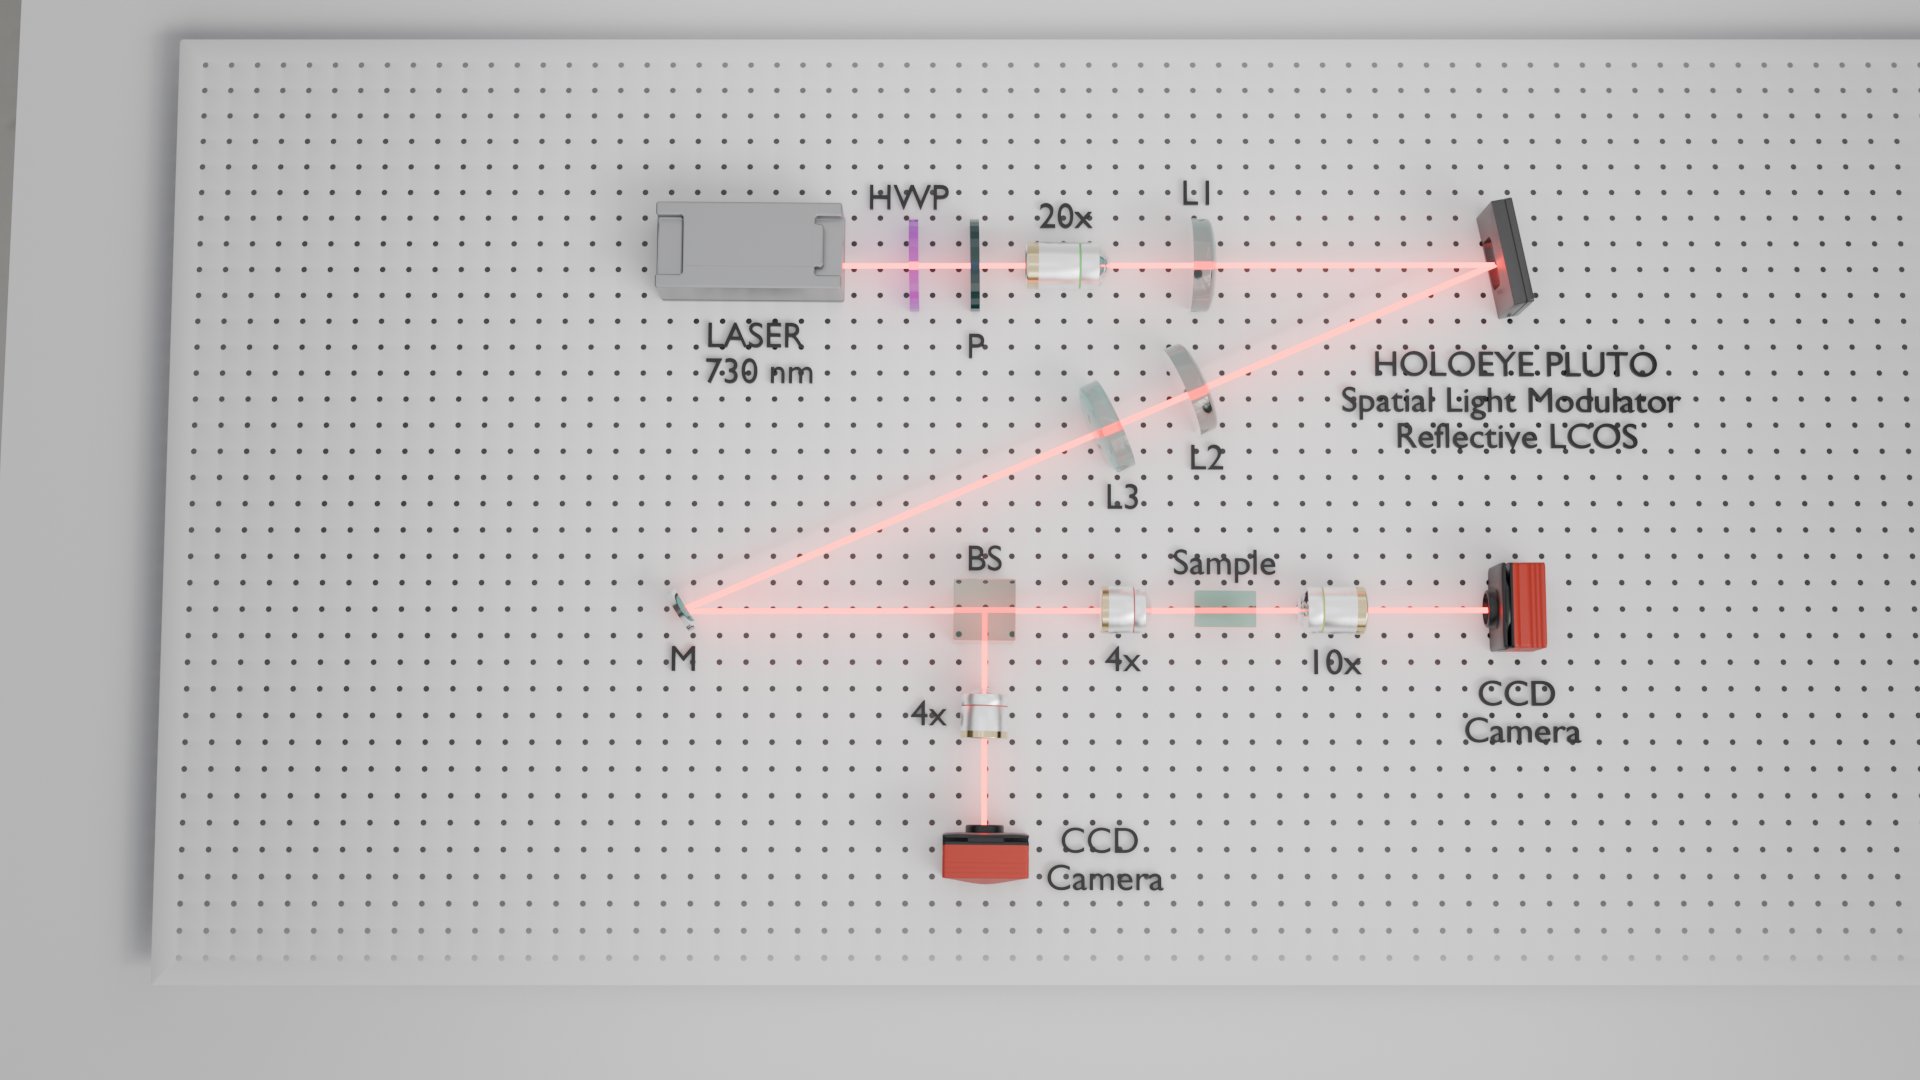
\includegraphics[width=0.8\linewidth, trim={21cm 5cm 7cm 5cm}, clip]{media/SLM_setupv1}
	\caption[Diagrama del sistema de modulación espacial de luz]{Diagrama completo del sistema experimental para modulación espacial de luz, mostrando los componentes ópticos y sus disposiciones relativas.}
	\label{fig:SLM_setup}
\end{figure}

\subsection{Generación de Imágenes Complejas \label{cap:oam}}
La capacidad de control preciso sobre amplitud y fase se verifica mediante la generación de vórtices ópticos, cuantificados por su Momentum Angular Orbital (OAM). El análisis interferométrico permite:
\begin{itemize}
	\item Determinar la carga topológica $\ell$ contando las ramas espirales en el patrón de interferencia.
	\item Establecer el signo de $\ell$ mediante la dirección de rotación del frente de fase.
\end{itemize}

\begin{figure}[H]
	\centering
	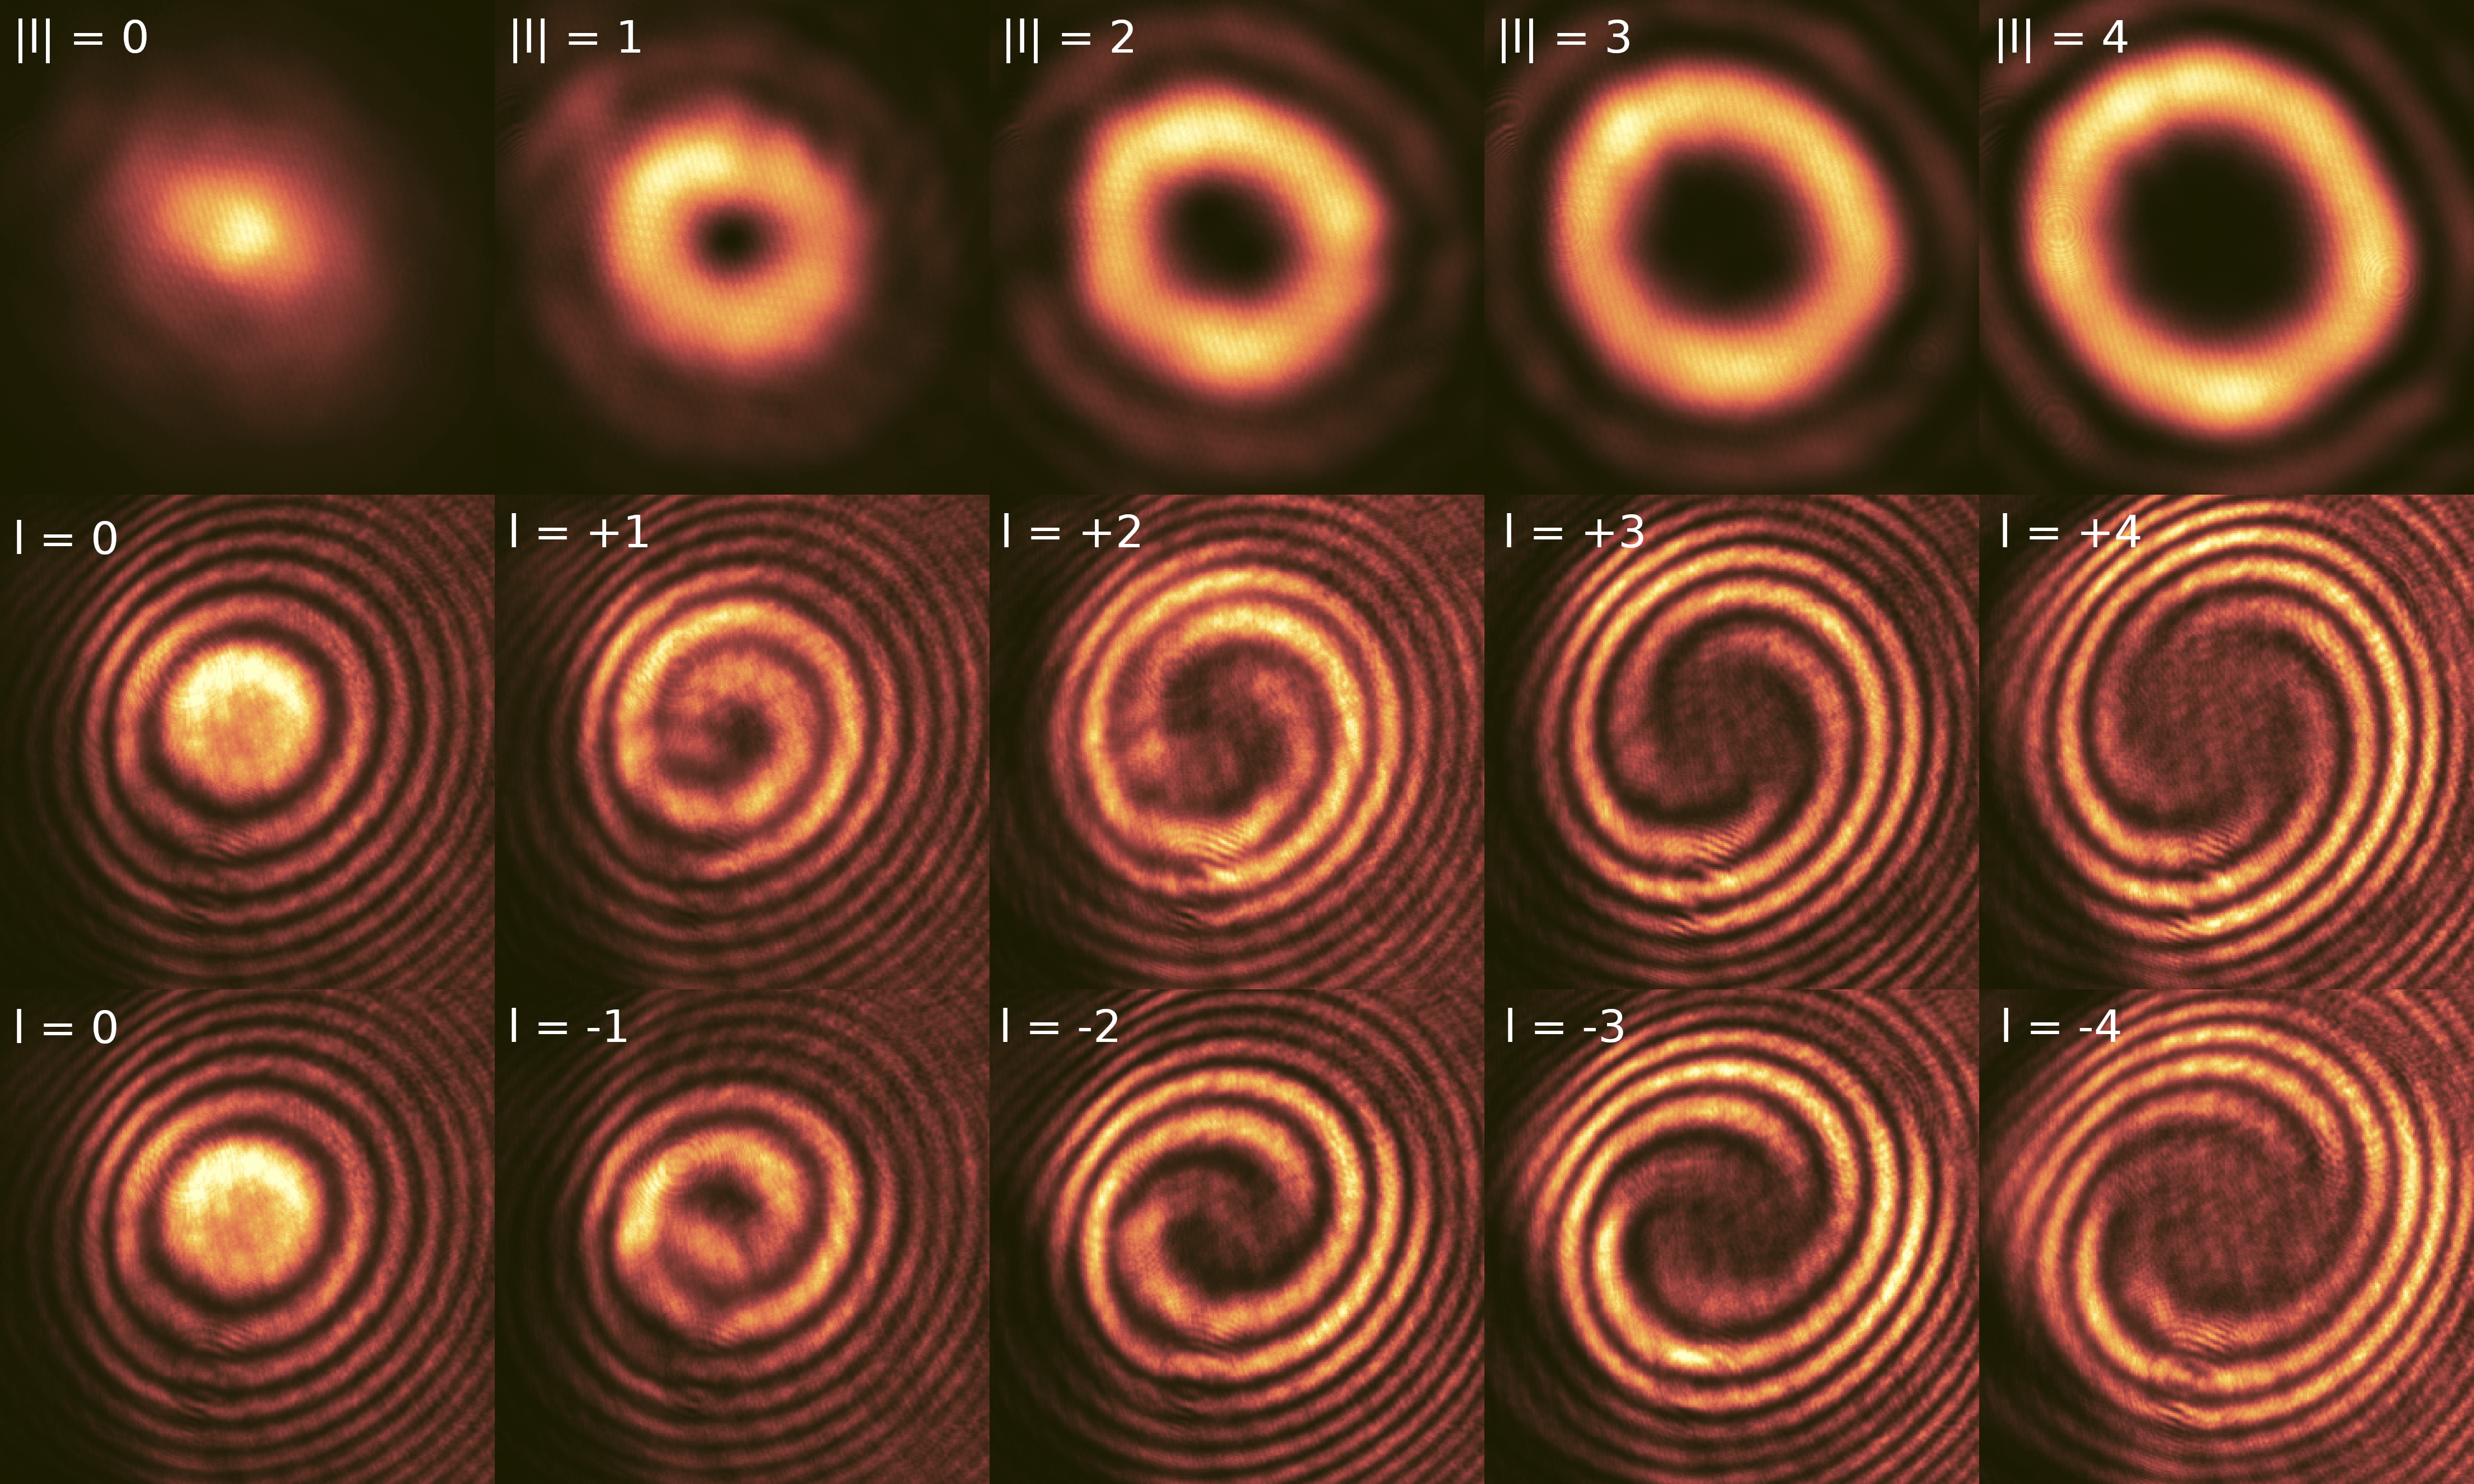
\includegraphics[width=0.95\linewidth]{media/OAM-free.png}
	\caption[Caracterización de vórtices ópticos mediante interferometría Mach-Zehnder.]{Caracterización de vórtices ópticos mediante interferometría Mach-Zehnder. \textbf{Arriba:} Intensidad para diferentes cargas OAM ($\ell$). \textbf{Centro y Abajo:} Patrones de interferencia correspondientes, donde el número de ramas espirales indica $|\ell|$ y el sentido de giro da cuenta del signo de $\ell$.}
	\label{fig:OAM}
\end{figure}
\section{Análisis de imágenes \label{sec:analimag}}
A partir de las imágenes capturadas es posible extraer información de la potencia que contiene cada sitio del sistema fotónico discreto en estudio. Para ello la imagen completa debe ser seccionada equispaciadamente en rectángulos que encierren las regiones donde existen guías de onda, iluminadas o no. La potencia de cada sitio será entonces la suma de la intensidad de cada píxel encerrado en su rectángulo respectivo.

El procesamiento de imágenes incluye:
\begin{itemize}
    \item Corrección de fondo
    \item Normalización por intensidad máxima.
    \item Segmentación automática mediante umbral.
\end{itemize}

Los datos obtenidos permiten reconstruir la distribución de potencia en la red fotónica y analizar fenómenos de acoplamiento entre guías vecinas.